\section{Resultados}
Nesta seção, será debatido acerca dos resultados obtidos por meio dos dois testes realizados. 

O primeiro visou analisar o tempo médio de cada algoritmo, bem como a sua variância. 

No segundo teste, por outro lado, buscou-se avaliar o comportamento dos algoritmos bolha e inserção quando submetidos a listas com diferentes taxas de ordenação, sendo elas 1\%, 3\%, 5\%, 10\% e, por fim, 50\%. 

Logo abaixo, têm-se os resultados em gráficos.

\subsection{Variação na quantidade de elementos}
Como comentado, os resultados comprovam o comportamento quadrático do bolha, seleção e inserção. 
Contudo, é necessário destacar que, caso houvesse uma maior variância nos números da lista a ser ordenada, isto é, caso a diferença entre o maior e o menor valor fosse um valor muito grande, o algoritmo de contagem apresentaria tempo para ordenar maior, podendo ultrapassar o bolha, por exemplo.

\begin{figure}[h]
    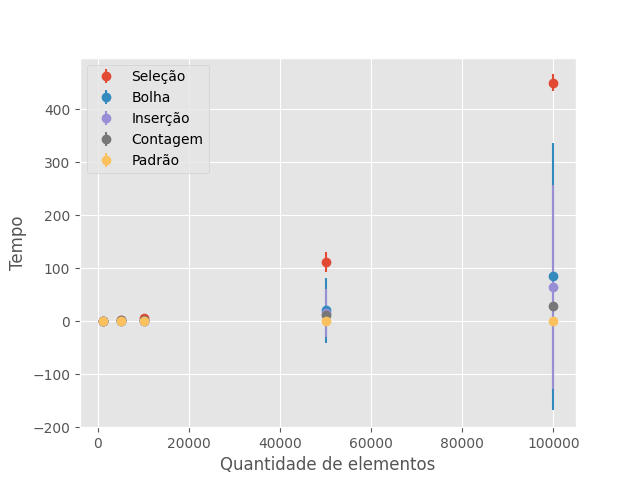
\includegraphics[width=8cm]{sizes.png}
    \caption{Gráfico elucidando o comportamento de cada algoritmo em tópico. No eixo x, há a quantidade de elementos; no eixo y, o tempo médio gasto em segundos}
    \end{figure}
    \newpage
    \subsection{Ordenação prévia}
    \begin{figure}[h]
        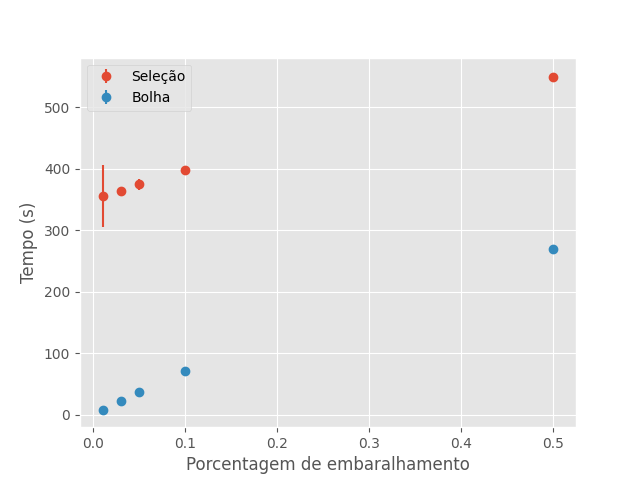
\includegraphics[width=8cm]{result_1717836837.057626.png}
        \caption{Gráfico ilustrando o tempo médio 'gasto' dos algoritmos bolha e inserção em relação à taxa de ordenação inicial dos vetores.}
    \end{figure}

O bolha, apesar de variar dependendo da taxa de ordenação, possui o maior tempo necessário para ordenar. Em seguida, o algoritmo de inserção detém o segundo maior tempo para ordenar, e isso se dá pelo fato de que o inserção possui uma complexidade quadrática independente da posição inicial dos elementos. 

O algoritmo de seleção, como esperado, contém o melhor tempo de resposta dentre os algoritmos de comparação, uma vez que, além de ser mais eficiente em listas com alguns elementos ordenados, realiza menos permutações que o bolha. 

Por último, o contagem apresentou o melhor desempenho dentre os implementados. Contudo, é necessário destacar que o contagem obteve este desempenho devido à faixa de números aleatórios escolhida (de 0 a 9999), pois, como analisado, o algoritmo em questão varia com os números recebidos.

Assim, percebe-se que, para listas com muitos elementos, o algoritmo contagem é o mais eficiente entre os implementados, enquanto o bolha apresentou o resultado menos satisfatório para o teste.

